Calculate the adjusted face by applying both brightness and contrast adjustments to make it as “good” as possible.

\begin{solution}\ 
    \begin{lstlisting}[language=Matlab]
    face_gray_adj = (255/(150-30))*(face_gray - 30);
    histogram(face_gray_adj);
    imshow(face_gray_adj);
    \end{lstlisting}

    \begin{center}
        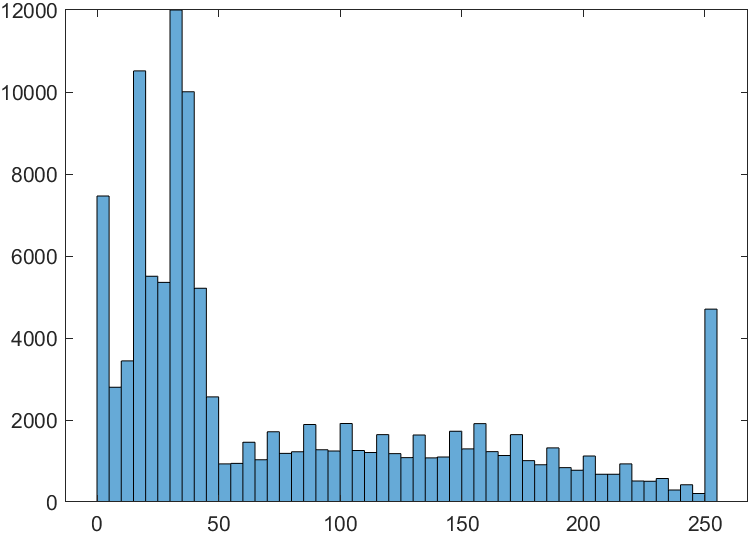
\includegraphics[width=0.8\textwidth]{img/e7p8c_hist.png}
    \end{center}

    \begin{center}
        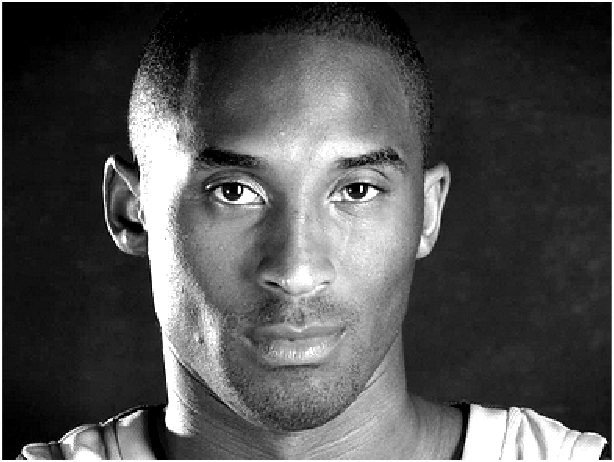
\includegraphics[width=0.5\textwidth]{img/e7p8c_img.png}
    \end{center}
    
    The contrast and intensity was adjusted to highlight the 30-150 range. 
\end{solution}